\section{Chandra Kirana Poetra}



 
 
\subsection{Sejarah python}

\begin{flushleft}
\qquad Python merupakan suatu bahasa pemrograman yang terinspirasi dari bahasa pemrograman ABC, bahasa pemrograman ABC inilah yang memengaruhi design dan juga pengembangan dari python. Dibuat oleh Guido Van Rossum pada tahun 1989 , python pada awalnya dikembangkan pada tahun 1980an pada saat Guido bekerja di CWI (Centrum voork Wiskunde en Informatica) sebagai programmer yang mengimplementasikan bahasa pemrograman bernama ABC, di sana dia mulai mencari bahasa seperti ABC tapi dengan akses mirip seperti AMOEBA, jadi Guido membuat sendiri bahasa pemrograman sederhana yang bisa menutup celah di ABC. Dan akhirnya pada tahun 1991, versi pertama dari python release ke publik
\end{flushleft}

\subsection{Instalasi Anaconda}
\begin{enumerate}
\item Pertama anda perlu mendownload terlebih dahulu anacondanya.
\item Visi link ini di https://www.anaconda.com/distribution/download-section
\item Setelah download anda selesai, buka file yang anda download tadi
\item Klik next
\begin{figure}[H]
\centering
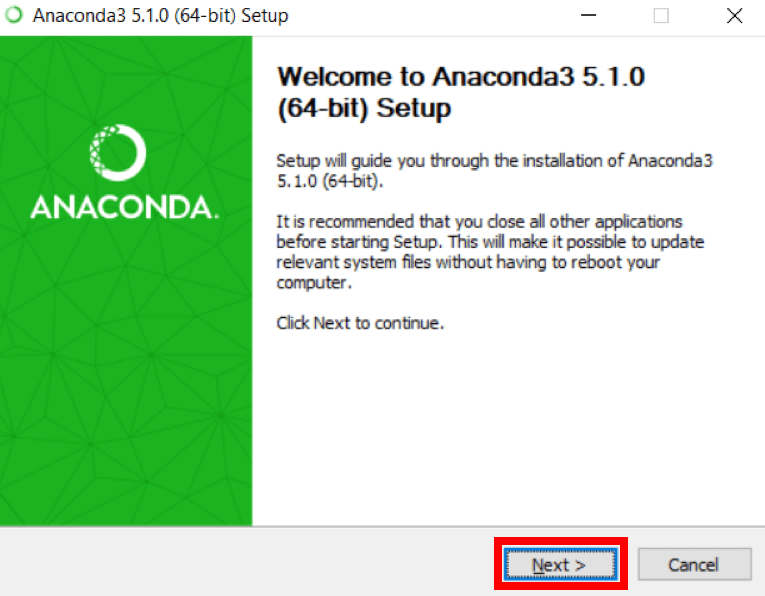
\includegraphics[width=6cm,height=6cm]{figures/1.png}
\caption{Klik Next}
\label{akhir}
\end{figure}
\item Klik I Agree
\begin{figure}[H]
\centering
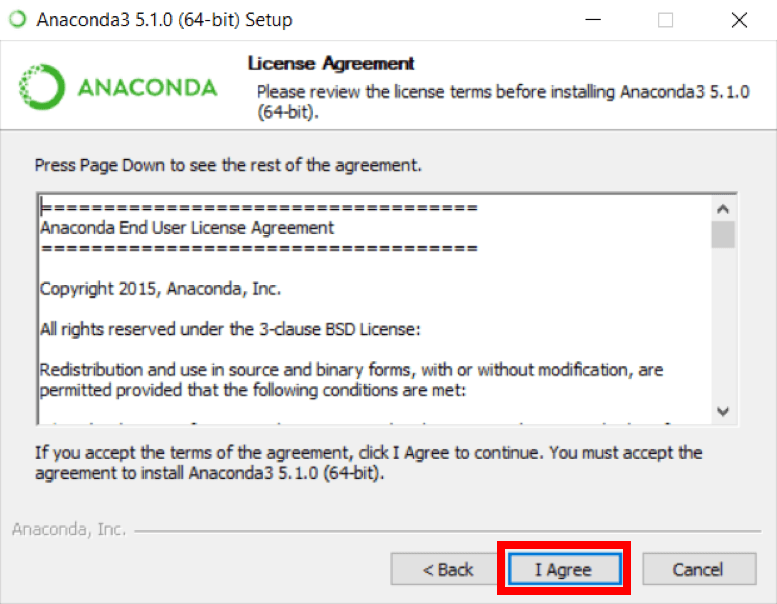
\includegraphics[width=6cm,height=6cm]{figures/2.png}
\caption{Klik I Agree}
\label{akhir}
\end{figure}
\item Pilih Just me dan klik next
\begin{figure}[H]
\centering
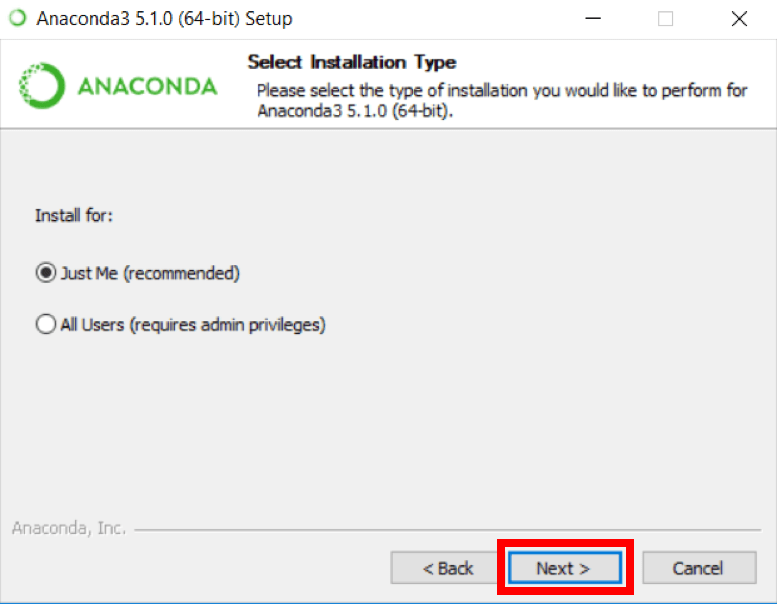
\includegraphics[width=6cm,height=6cm]{figures/3.png}
\caption{Pilih just me saja}
\label{akhir}
\end{figure}
\item Pilih directory tempat anaconda akan diinstal lalu next
\begin{figure}[H]
\centering
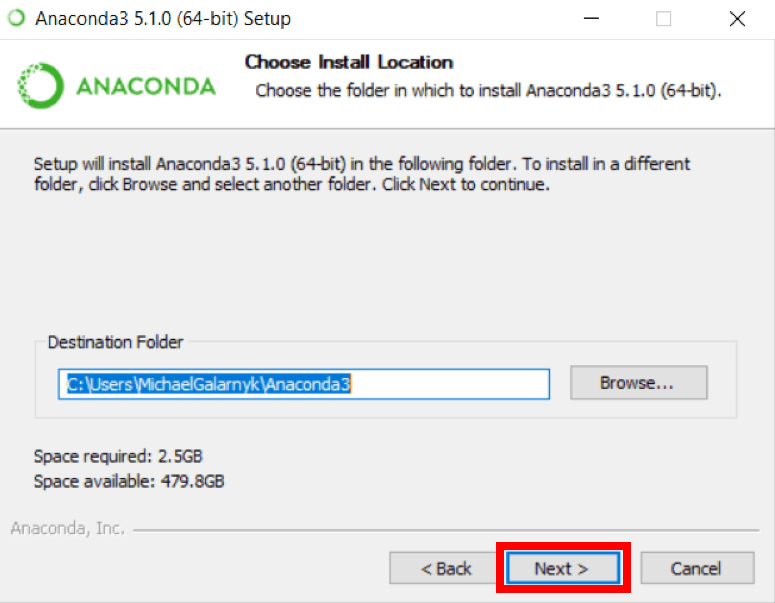
\includegraphics[width=6cm,height=6cm]{figures/4.png}
\caption{Directory tempat anaconda akan diinstalt}
\label{akhir}
\end{figure}
\item Pilih hanya opsi yang bawah saja
\begin{figure}[!htbp]
\centering
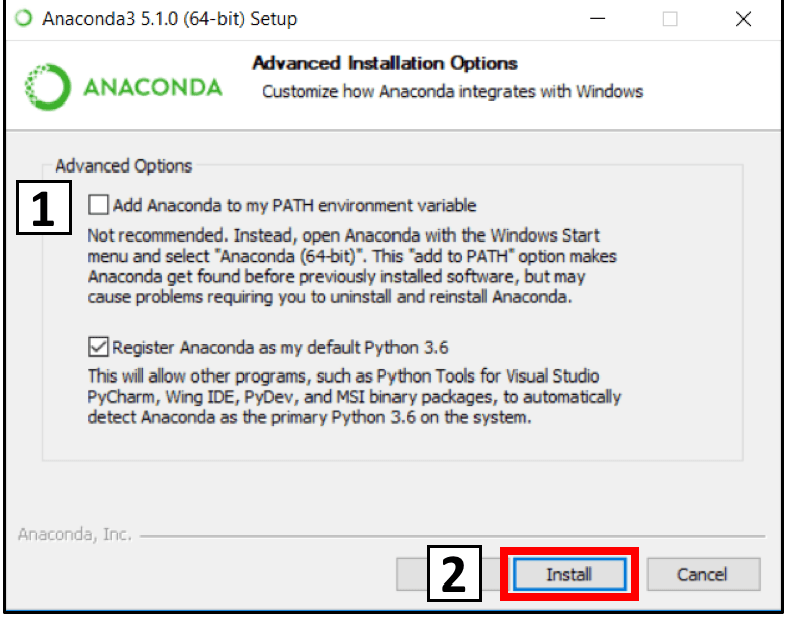
\includegraphics[width=6cm,height=6cm]{figures/5.png}
\caption{Opsi Register}
\label{akhir}
\end{figure}
\item Tunggu hingga proses selesai lalu next
\begin{figure}[H]
\centering
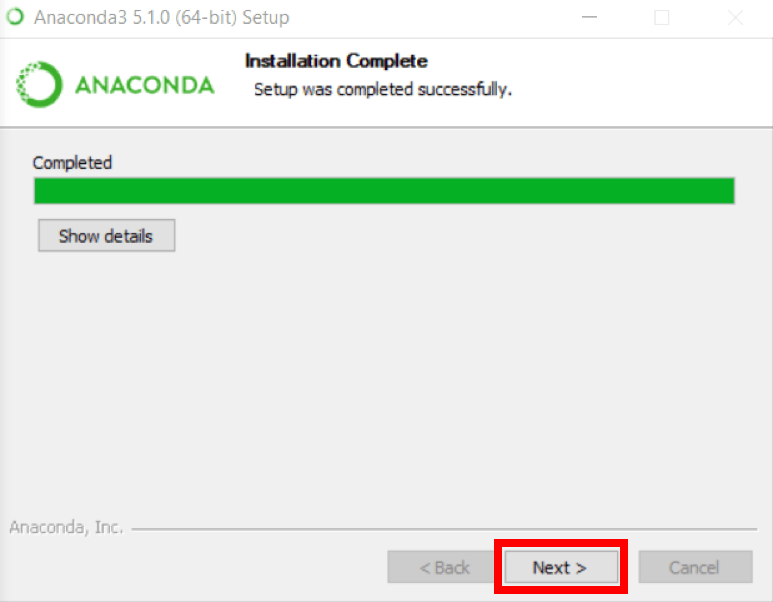
\includegraphics[width=6cm,height=6cm]{figures/6.png}
\caption{Tunggu hingga selesai}
\label{akhir}
\end{figure}
\item Opsi tambahan untuk instal visual studio code, skip saja
\begin{figure}[H]
\centering
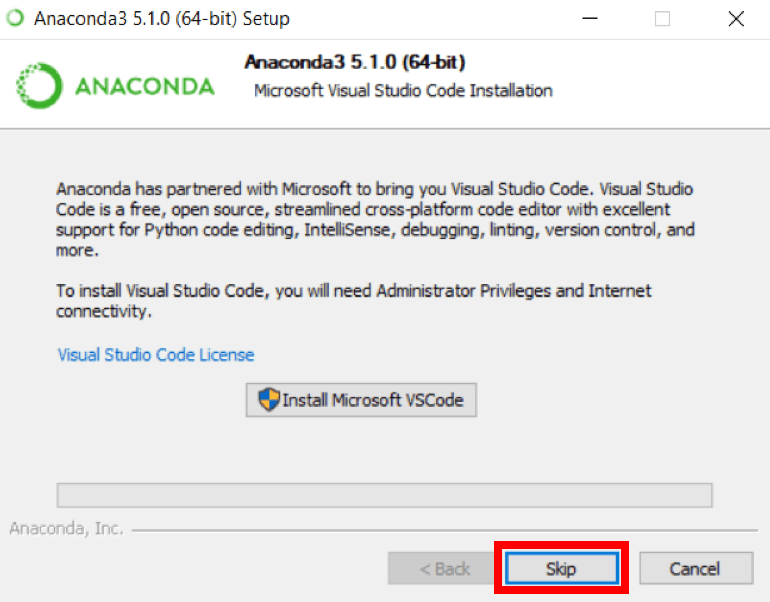
\includegraphics[width=6cm,height=6cm]{figures/7.png}
\caption{Opsi Tambahan}
\label{akhir}
\end{figure}
\item Klik saja finish
\begin{figure}[H]
\centering
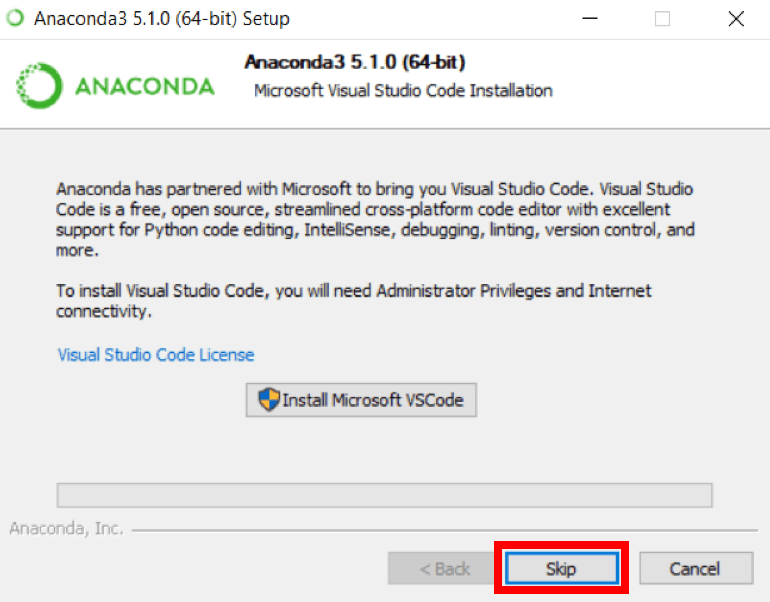
\includegraphics[width=6cm,height=6cm]{figures/7.png}
\caption{Finish}
\label{akhir}
\end{figure}
\end{enumerate}

\subsection{Spyder}
\begin{enumerate}
\item Setelah tadi install anaconda, buka aplikasinya.
\item Biasanya, spyder sudah terinstall bersamaan dengan anaconda, klik launch pada spyder
\begin{figure}[H]
\centering
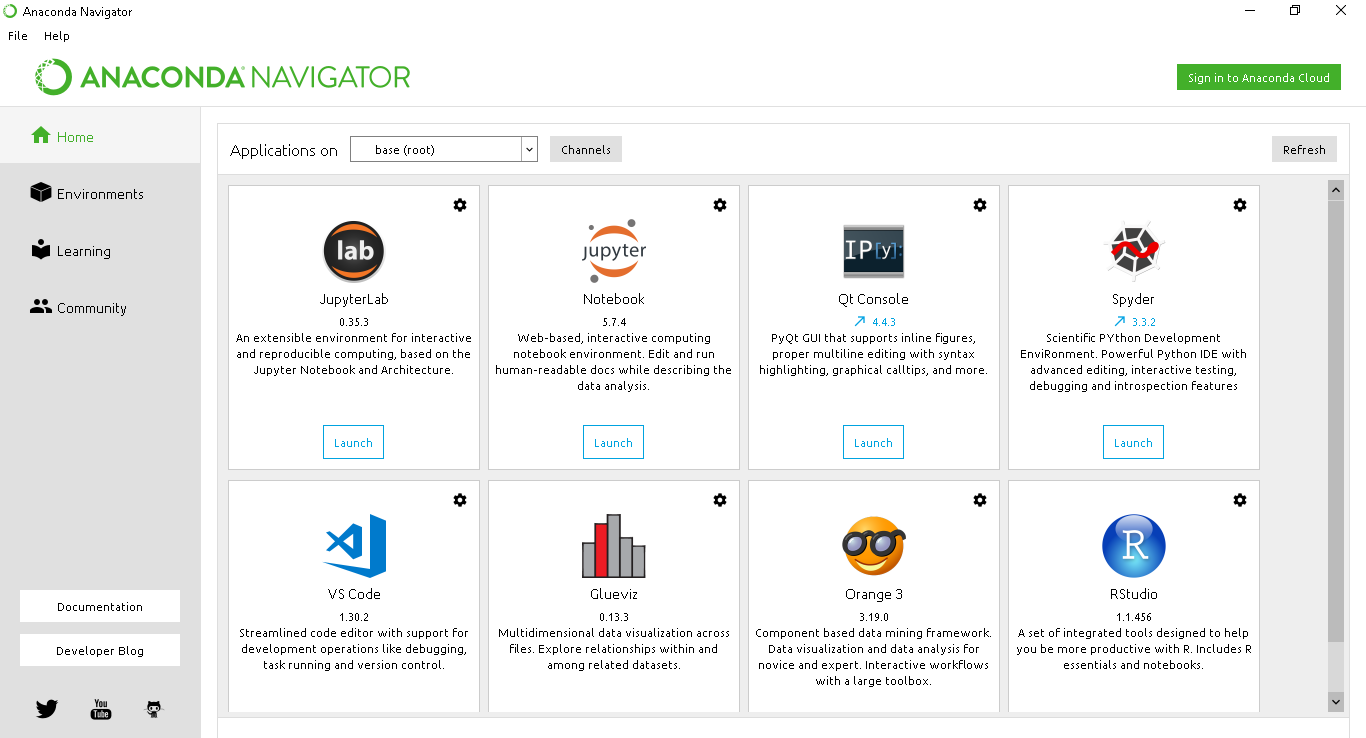
\includegraphics[width=6cm,height=6cm]{figures/9.png}
\caption{Tampilan awal anaconda}
\label{akhir}
\end{figure}
\item ketika di menu kiri, print("Hellow World") untuk percobaan pertama lalu klik simbo panah hijau untuk run, maka anda akan melihat hasilnya di console
\begin{figure}[H]
\centering
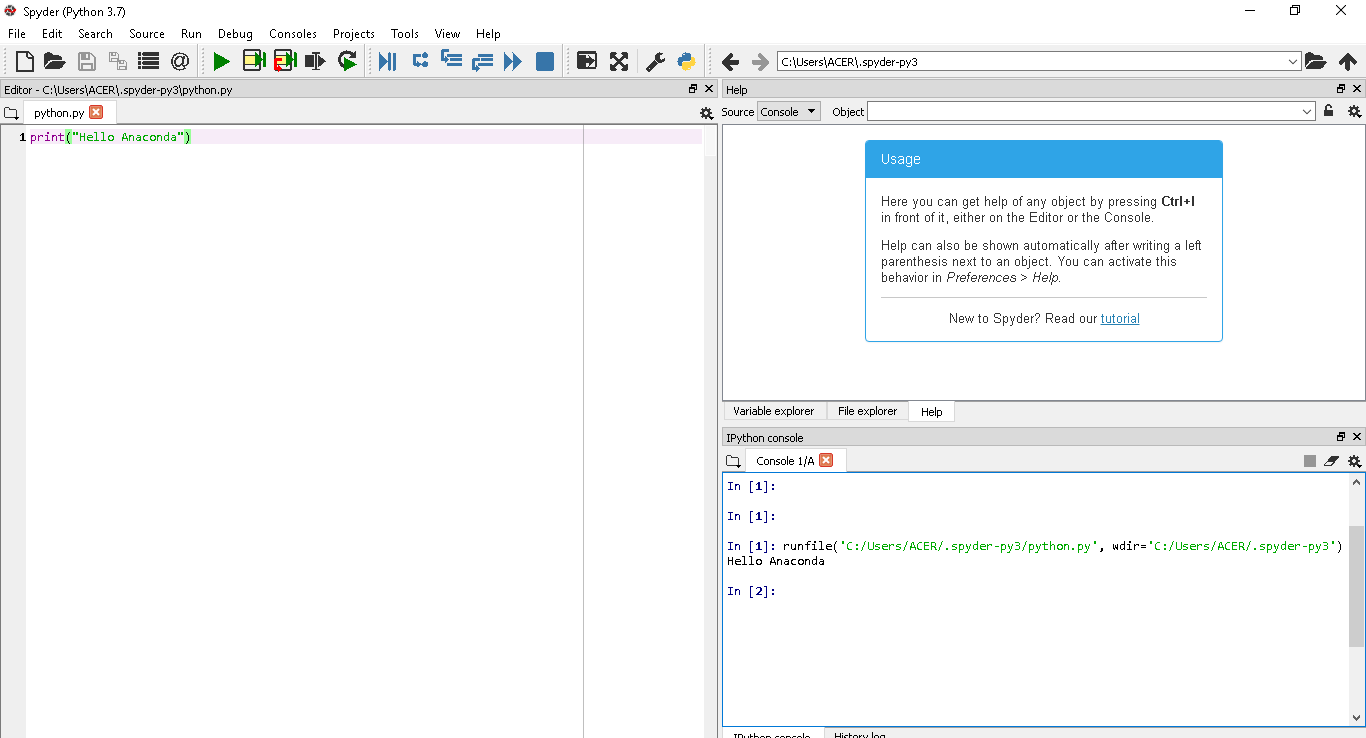
\includegraphics[width=6cm,height=6cm]{figures/10.png}
\caption{IDE Spyder}
\label{akhir}
\end{figure}

\item Output akan dihasilkan di sini
\begin{figure}[H]
\centering
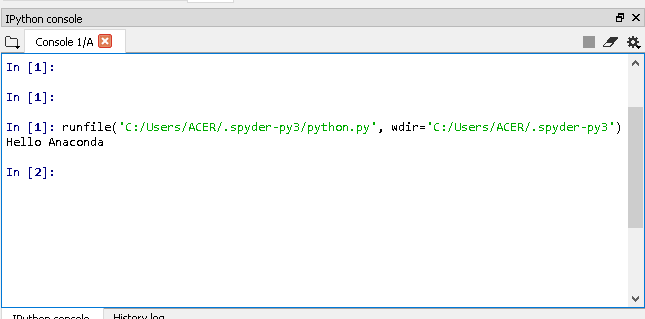
\includegraphics[width=6cm,height=6cm]{figures/11.png}
\caption{Menu Console}
\label{akhir}
\end{figure}


\end{enumerate}
